\section{Forward problem appendix}
\subsection{Head models}

\begin{figure}[!htbp]
    \centering
    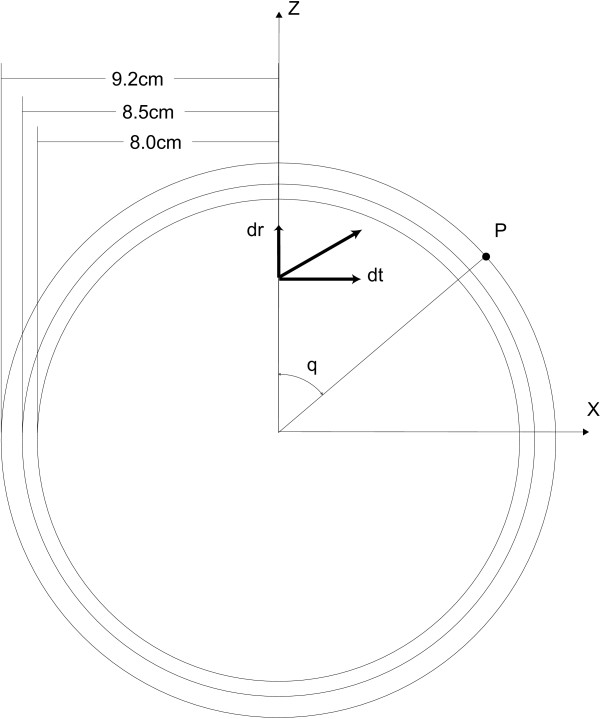
\includegraphics[width=0.4\textwidth]{HeadModel.jpg}
    \caption{Spherical head model}\label{Fig4}
\end{figure}

\begin{figure}[!htbp]
    \centering
    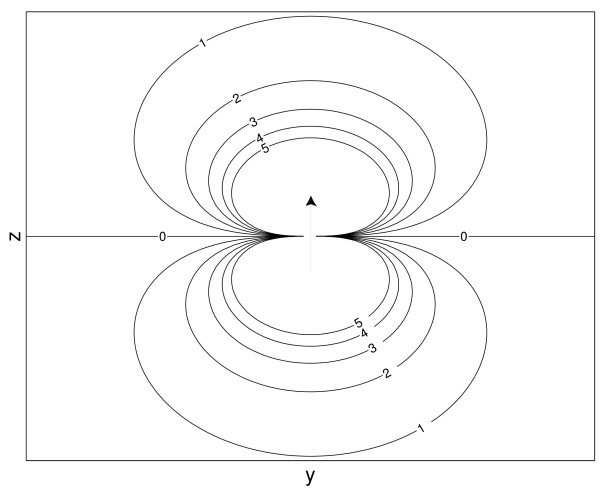
\includegraphics[width=0.4\textwidth]{Electrical_field.jpg}
    \caption{Dipole electrical field}\label{Fig7}
\end{figure}




\begin{figure}[!htbp]
    \centering
    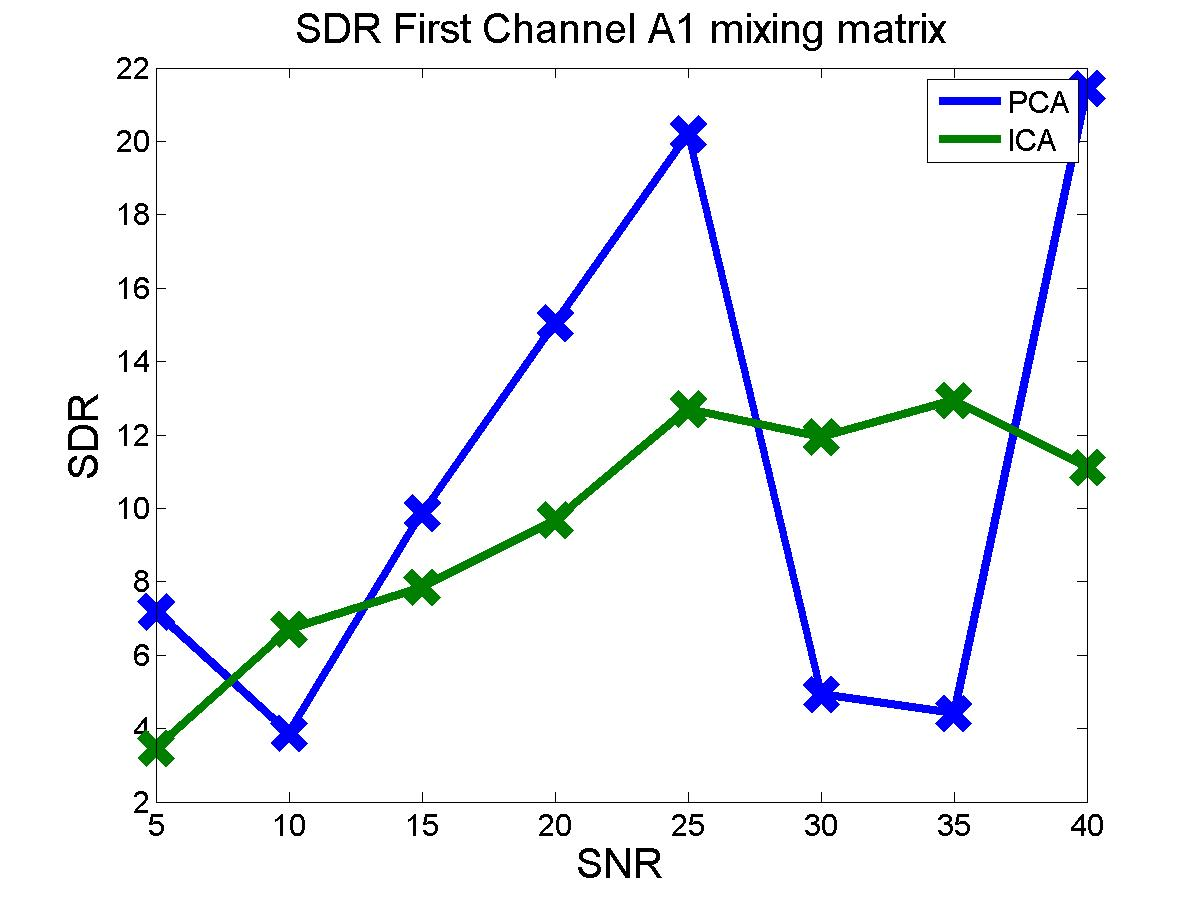
\includegraphics[width=0.3\textwidth]{1.png}
    \caption{Dipole modeling}
\end{figure}

\begin{figure}[!htbp]
    \centering
    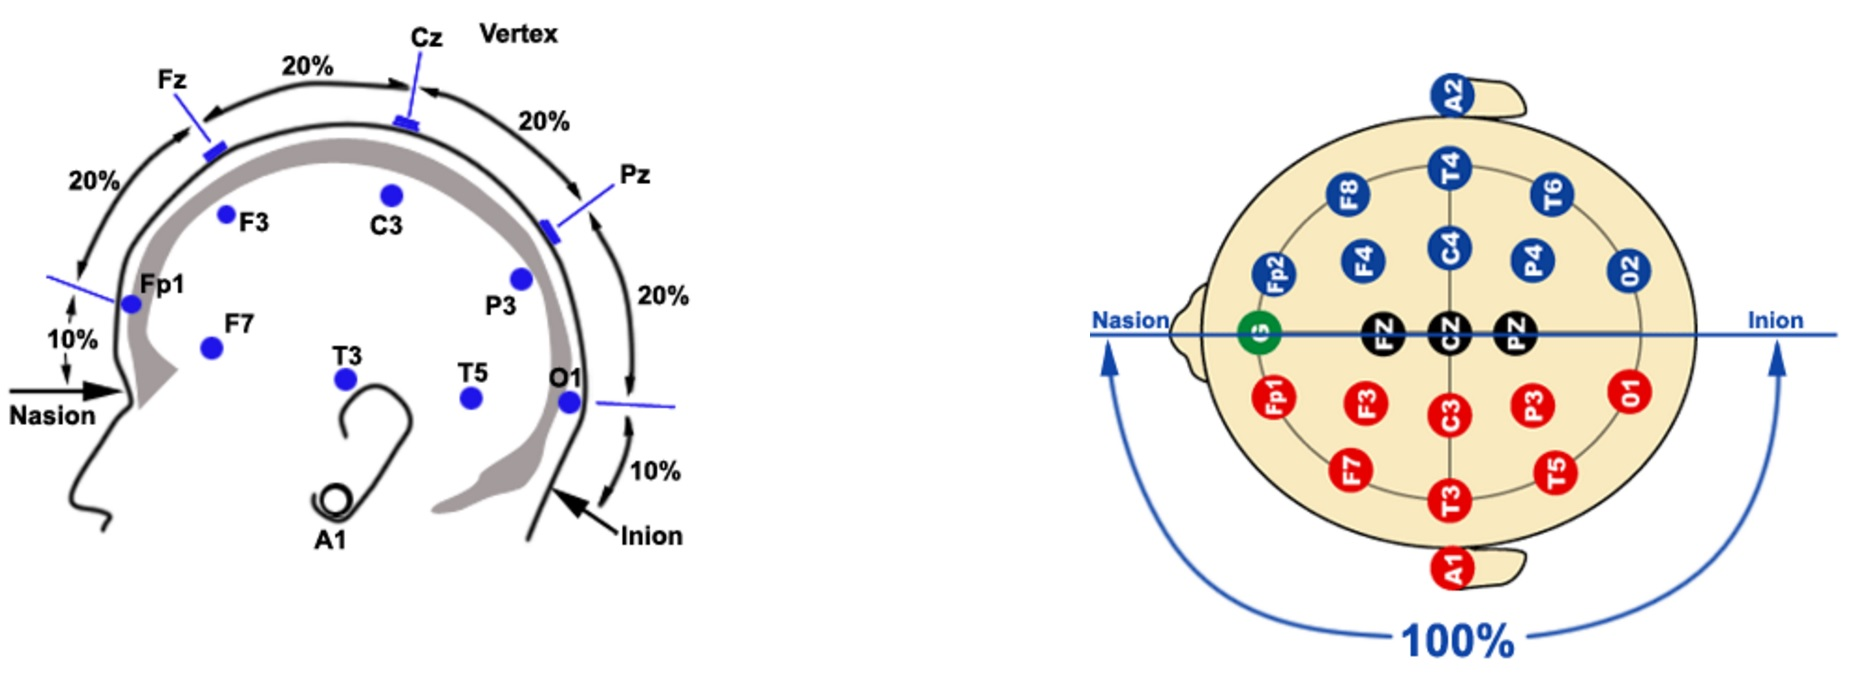
\includegraphics[width=1\textwidth]{ElectrodPlacement.jpg}
    \caption{EEG montage}
    \label{Fig1}
\end{figure}

\newpage
\subsection{The Potential of a General Dipole}\label{Ap1}



Consider a dipole with a dipole moment ${\vec{D}}=(D_x,D_y,D_z)$ located at ${\vec{R_1}}=(X_1,Y_1,Z_1)$, and a point on the scalp ${\vec{R_2}}=(X_2,Y_2,Z_2)$. The radius vectors $\vec{R_1}$ and $\vec{R_2}$ define a plane in space, which will be called the major plane. The cross product ${\vec{N}=\vec{R_1} \times \vec{R_2}}$ is perpendicular to the major plane. The cross product ${\vec{t}=\vec{N} \times \vec{R_1}}$ is in the major plane, and perpendicular to ${\vec{R_1}}$. Based on an identity from algebra, ${\vec{t}=\vec{R_2}(\vec{R_1} \cdot \vec{R_1})-\vec{R_1}(\vec{R_1} \cdot \vec{R_2})}$, or by components



\begin{figure}[!htbp]
\minipage{0.3\textwidth}%
\centering
\begin{equation}
t_x=X_2 \cdot p-X_1 \cdot q
\end{equation}
\endminipage\hfill
\minipage{0.3\textwidth}%
\centering
\begin{equation}
t_y=Y_2 \cdot p-Y_1 \cdot q
\end{equation}
\endminipage\hfill
\minipage{0.3\textwidth}%
\centering
\begin{equation}
 t_z=Z_2 \cdot p-Z_1 \cdot q
\end{equation}
\endminipage\hfill
\end{figure}






where ${p}={X_1}^2+{Y_1}^2+{Z_1}^2$ and ${q}=X_1 \cdot X_2+Y_1 \cdot Y_2+Z_1 \cdot Z_2$.
$\vec{T}=(T_x,T_y,T_z)$ is the unit vector in the ${\vec{t}}$ direction, which is the tangential direction to $\vec{R_1}$ in the major plane. Its components are 


\begin{figure}[!htbp]
\minipage{0.3\textwidth}%
\centering
\begin{equation}
 T_x=t_x/|t|
\end{equation}
\endminipage\hfill
\minipage{0.3\textwidth}%
\centering
\begin{equation}
 T_y=t_y/|t|
\end{equation}
\endminipage\hfill
\minipage{0.3\textwidth}%
\centering
\begin{equation}
 T_z=t_z/|t|
\end{equation}
\endminipage\hfill
\end{figure}




where $|t|={({t_x}^2+{t_y}^2+{t_z}^2)}^{1/2}$.
The unit vector ${\overrightarrow{RR}}=(R_x,R_y,R_z)$ in the radial direction $\vec{R_1}$ is 


\begin{figure}[!htbp]
\minipage{0.3\textwidth}%
\centering
\begin{equation}
 R_x=X_1/|\vec{R_1}|
\end{equation}
\endminipage\hfill
\minipage{0.3\textwidth}%
\centering
\begin{equation}
 R_y=Y_1/|\vec{R_1}|
\end{equation}
\endminipage\hfill
\minipage{0.3\textwidth}%
\centering
\begin{equation}
 R_z=Z_1/|\vec{R_1}|
\end{equation}
\endminipage\hfill
\end{figure}




where $|\vec{R_1}|={({X_1}^2+{Y_1}^2+{Z_1}^2)}^{1/2}$.
The cosine of the angle between $\vec{R_1}$ and $\vec{R_2}$ is 
\begin{equation}\label{new_label}
 cos\alpha=q/|\vec{R_1}|\cdot|\vec{R_2}|
\end{equation}
where $|\vec{R_2}|={({X_2}^2+{Y_2}^2+{Z_2}^2)}^{1/2}$.
The potential that the dipole $\vec{D}$ generates at the scalp point $\vec{R_2}$ is the sum of the potentials contributed by $D_x$, $D_y$ and $D_z$. When these expressions are substituted in equation \ref{eq11} the potential at $\vec{R_2}$ due to $D_x$ turns to be 
\begin{equation}
 V_x=\bigg\{ \frac{1}{4\pi S{R}^2}\displaystyle\sum_{i=1}^{\infty} \frac{X(2n+1)^3}{d_n(n+1)n}}.{b}^{n-1}\{nR_xP_n(cos\alpha)+T_x{P_n}^1(cos\alpha)\}\bigg\}D_x
\end{equation}


and similarly, the potential due to $D_y$ and $D_z$ would be 
\begin{equation}
 V_y=\bigg\{ \frac{1}{4\pi S{R}^2}\displaystyle\sum_{i=1}^{\infty} \frac{X(2n+1)^3}{d_n(n+1)n}}.{b}^{n-1}\{nR_yP_n(cos\alpha)+T_y{P_n}^1(cos\alpha)\}\bigg\}D_y
\end{equation}


\begin{equation}
 V_z=\bigg\{ \frac{1}{4\pi S{R}^2}\displaystyle\sum_{i=1}^{\infty} \frac{X(2n+1)^3}{d_n(n+1)n}}.{b}^{n-1}\{nR_zP_n(cos\alpha)+T_z{P_n}^1(cos\alpha)\}\bigg\}D_z
\end{equation}


where ${b}=|\vec{R_1}|/R$< and $cos\alpha$ is given by equation \ref{new_label}. The potential $V$ at $\vec{R_2}$ due to $\vec{D}$ at $\vec{R_1}$ is ${V}=V_x+V_y+V_z$.
Assigning a Reference Electrode 

1) An arbitrary convenient point on the surface, denoted by $\vec{R_0}$, is declared as the reference. All potentials are measured with respect to the electrode at this point. 
(If the potentials have already been measured with respect to a different point, such as left earlobe, they have to be adjusted accordingly. The measured potential at $\vec{R_0}$ (with respect to the earlobe) should be subtracted from the measured potential at each point). 

2) Equations \ref{new_label1} are corrected for the new reference point, and become


\begin{figure}[!htbp]
\minipage{0.3\textwidth}%
\centering
\begin{equation}
 {V_x}'=(T_{x12}-T_{x10}).D_x
\end{equation}
\endminipage\hfill
\minipage{0.3\textwidth}%
\centering
\begin{equation}
 {V_y}'=(T_{y12}-T_{y10}).D_y
\end{equation}
\endminipage\hfill
\minipage{0.3\textwidth}%
\centering
\begin{equation}
 {V_z}'=(T_{z12}-T_{z10}).D_z
\end{equation}
\endminipage\hfill
\end{figure}




where $T_{xl0}$, $T_{yl0}$, $T_{zl0}$ are the transfer coefficients from a dipole at $\vec{R_1}$ onto surface point $\vec{R_0}$. $V'$, the theoretical potential at $\vec{R_2}$ with respect to $\vec{R_0}$ due to a dipole at $\vec{R_1}$ is given by 
\begin{equation}
 {V}'={V_X}'+{V_Y}'+{V_Z}'.
\end{equation}